%%%%%%%%%%%%%%%%%%%%%%%%%%%%%%%%%%%%%%%%%%%%%%%%%%%%%%%%%%%%%%
\fe{\section{Compléments}}{\section{Supplements}}
\label{complements}
%%%%%%%%%%%%%%%%%%%%%%%%%%%%%%%%%%%%%%%%%%%%%%%%%%%%%%%%%%%%%%

\fe{\subsection{Éléments poutres/coques 3D/2D/1D}}{\subsection{Beam/Shell Elements 3D/2D/1D}}
\begin{frame}{\fe{Fichiers solution}{Solution files}}
  \begin{itemize}
    \item \fe{Les fichiers solution de cette formation sont des cas tests\\
              téléchargeables sur le site web :}
             {The solution files of this tutorial are in the examples base\\
              download them from the web site:}\\~\\
    \begin{center}
      \url{https://www-cast3m.cea.fr/index.php?page=exemples}\\~\\
    \end{center}
    $\Rightarrow$~formation\_debutant\_1\_maillage.dgibi\\
    $\Rightarrow$~formation\_debutant\_2\_thermique.dgibi\\
    $\Rightarrow$~formation\_debutant\_3\_mecanique.dgibi
  \end{itemize}
\end{frame}

\begin{frame}{\fe{Éléments finis barre/poutre, coque, joints...}
                 {Truss/beam, shell, joint... finite elements}}
  \begin{itemize}
    \item \fe{Le choix des éléments finis se fait dans \kwr{MODE}}
             {The choice of finite element must be made in \kwr{MODE}}
    \lstinputlisting[language=gibiane, firstline=29, lastline=33]{dgibi/exemples.dgibi}
    \item \fe{Les caractéristiques géométriques sont données dans \kwr{MATE}}
             {Geometrical characteristics are given in \kwr{MATE}}
    \lstinputlisting[language=gibiane, firstline=34, lastline=37]{dgibi/exemples.dgibi}
    \item \fe{On peut alors agir sur les d.d.l. de déplacement et de rotation}
             {Then you can prescribe d.o.f. for displacements and rotation}
    \lstinputlisting[language=gibiane, firstline=38, lastline=38]{dgibi/exemples.dgibi}
  \end{itemize}
\end{frame}

\begin{frame}{\fe{Éléments finis barres en 3D}{Truss finite elements in 3D}}
  \begin{itemize}
    \item \fe{Exemple d'un treillis de barres type grue (en 3D)}
             {Example of a lattice truss crane (in 3D)}
    \begin{textblock*}{6cm}(7cm,0cm)
      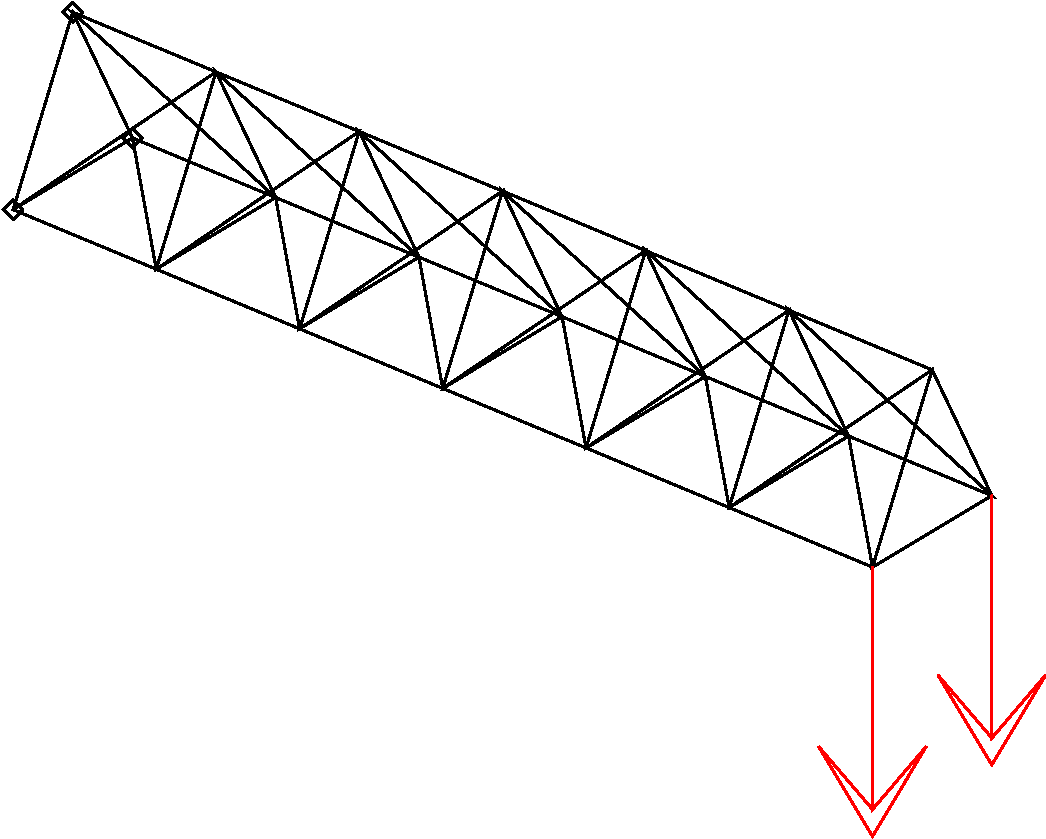
\includegraphics[width=4.5cm]{images/treillis_grue_3d.1}
    \end{textblock*}
    \begin{textblock*}{6cm}(7cm,2.5cm)
      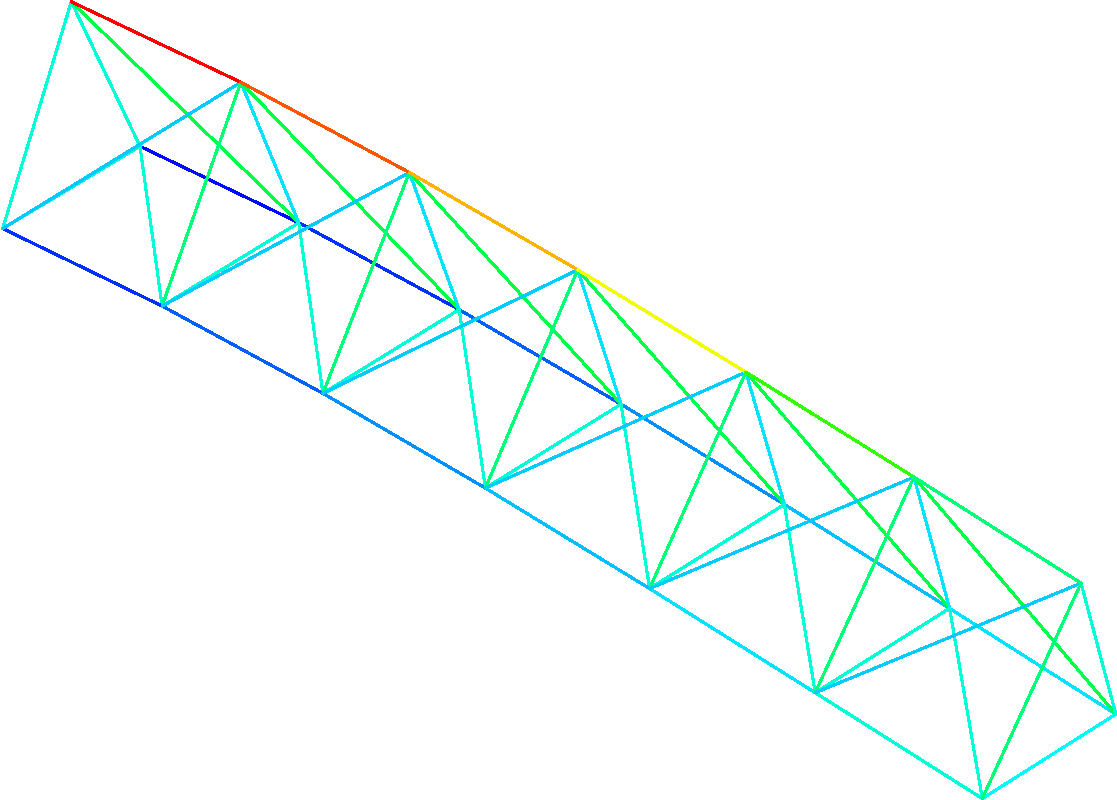
\includegraphics[width=4.5cm]{images/treillis_grue_3d.2}
    \end{textblock*}
    \lstinputlisting[basicstyle=\ttfamily\tiny, language=gibiane, firstline=2, lastline=28]{dgibi/treillis_grue_3d.dgibi}
  \end{itemize}
  \vspace{1cm}
\end{frame}

\begin{frame}{\fe{Éléments finis coques en 3D}{Shell finite elements in 3D}}
  \begin{itemize}
    \item \fe{Exemple d'une coque cylindrique sous pression (en 3D)}
             {Example of a cylindrical shell under pressure (in 3D)}
    \begin{textblock*}{6cm}(7.8cm,0.2cm)
      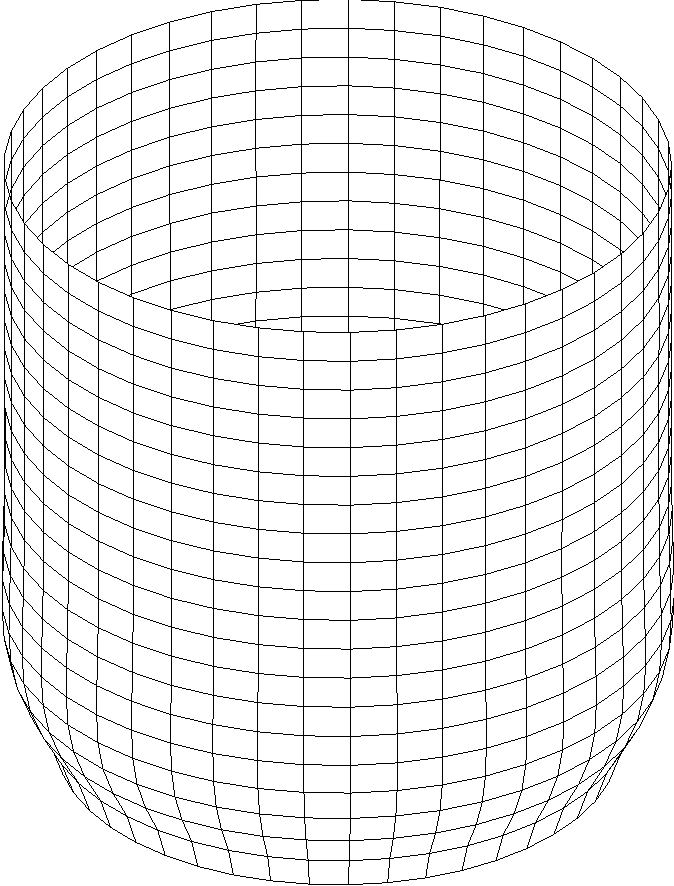
\includegraphics[height=5.5cm]{images/coque_3d}
    \end{textblock*}
    \lstinputlisting[basicstyle=\ttfamily\tiny, language=gibiane, firstline=25, lastline=40]{dgibi/coque_2d_axi_3d.dgibi}
  \end{itemize}
  \vspace{1cm}
\end{frame}

\begin{frame}{\fe{Éléments finis coques en 2D}{Shell finite elements in 2D}}
  \begin{itemize}
    \item \fe{Le même cas en 2D (axisymétrique)}{The same case in 2D (axisymmetric)}
    \begin{textblock*}{6cm}(9.5cm,0.2cm)
      
\includegraphics[height=5.5cm]{images/coque_2d_axi}
    \end{textblock*}
    \lstinputlisting[basicstyle=\ttfamily\tiny, language=gibiane, firstline=5, lastline=20]{dgibi/coque_2d_axi_3d.dgibi}
  \end{itemize}
  \vspace{1cm}
\end{frame}

\begin{frame}{\fe{Et d'autres options (2D, 1D, ...)}{And some other options (2D, 1D, ...)}}
  \begin{itemize}
    \item \fe{Exemple d'un problème de conduction stationnaire axisymétrique}
             {Example of steady state axisymmetric conduction problem}
    \begin{textblock*}{6cm}(7.2cm,-0.4cm)
      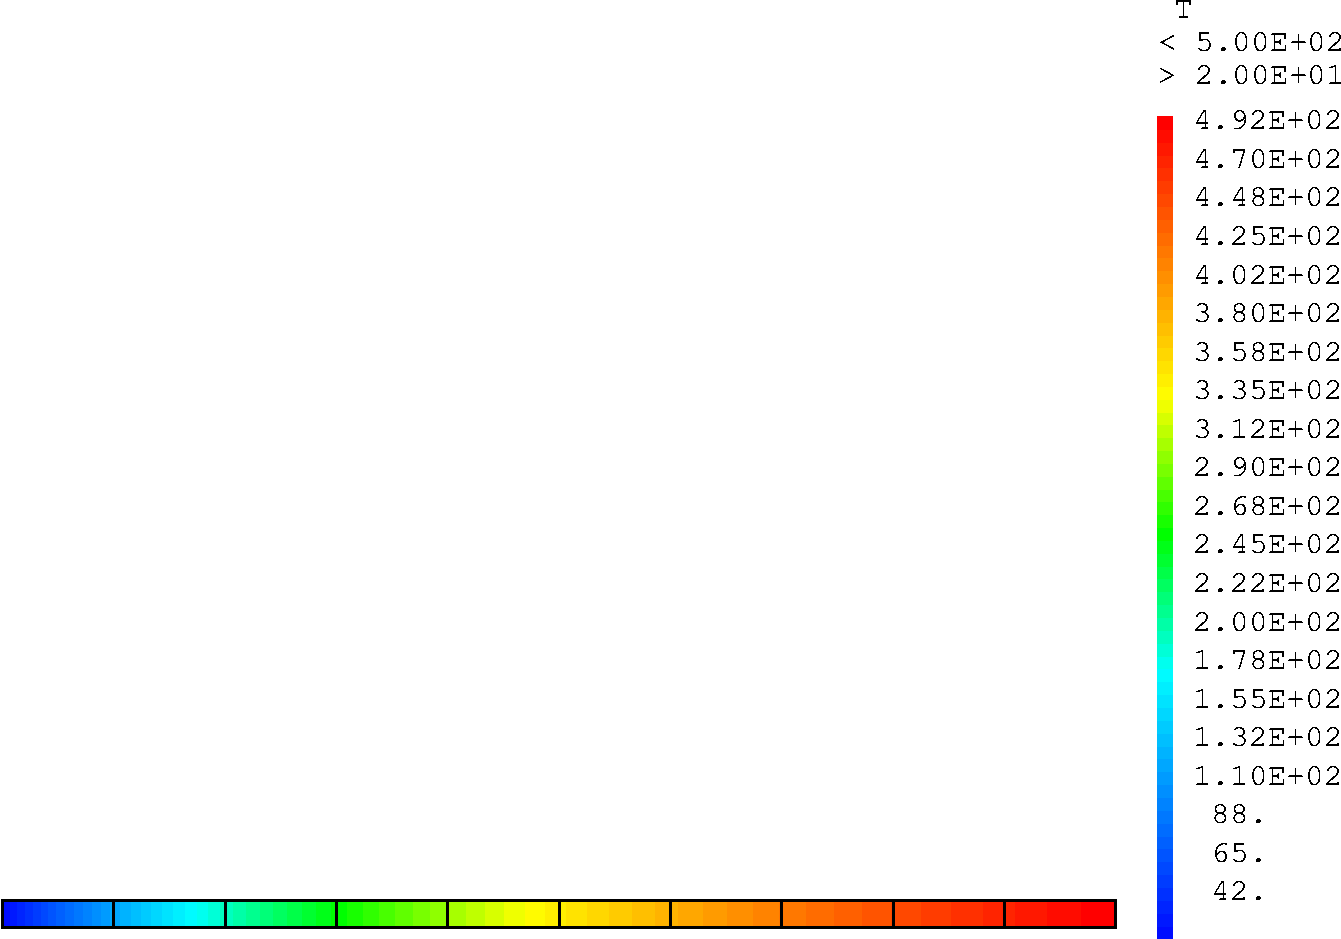
\includegraphics[width=5cm]{images/thermique_2d_axi.1}
    \end{textblock*}
    \begin{textblock*}{6cm}(6.8cm,3.5cm)
      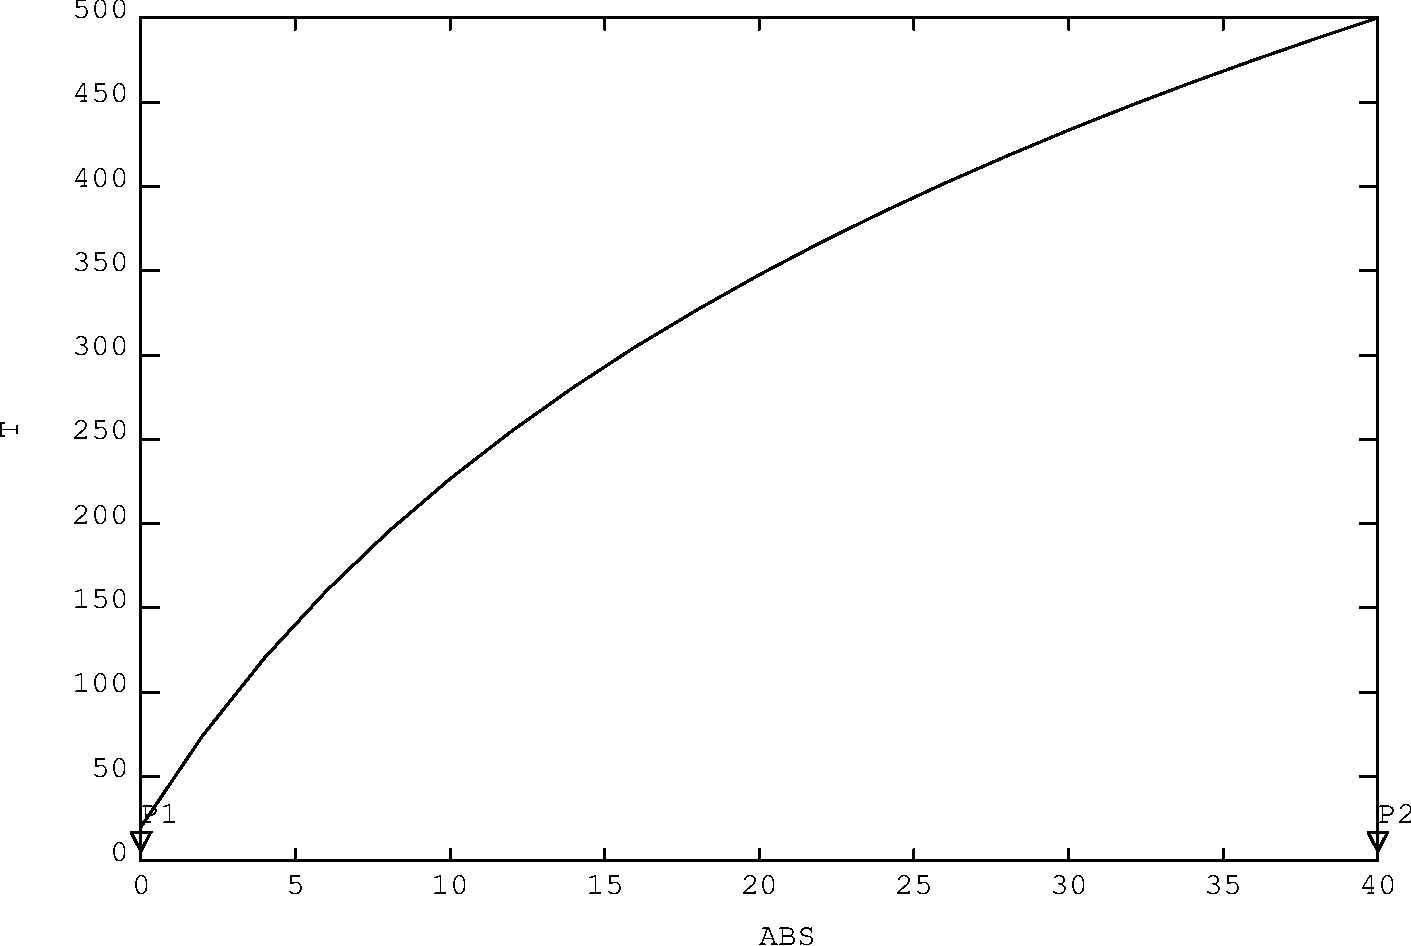
\includegraphics[width=5cm]{images/thermique_2d_axi.2}
    \end{textblock*}
    \lstinputlisting[basicstyle=\ttfamily\tiny, language=gibiane, firstline=31, lastline=52]{dgibi/thermique_1d_2d_axi.dgibi}
  \end{itemize}
  \vspace{1cm}
\end{frame}

\begin{frame}{\fe{Et d'autres options (2D, 1D, ...)}{And some other options (2D, 1D, ...)}}
  \begin{itemize}
    \item \fe{Le même cas en 1D (cylindrique)}{The same case in 1D (cylindrical)}
    \begin{textblock*}{6cm}(7.2cm,-0.4cm)
      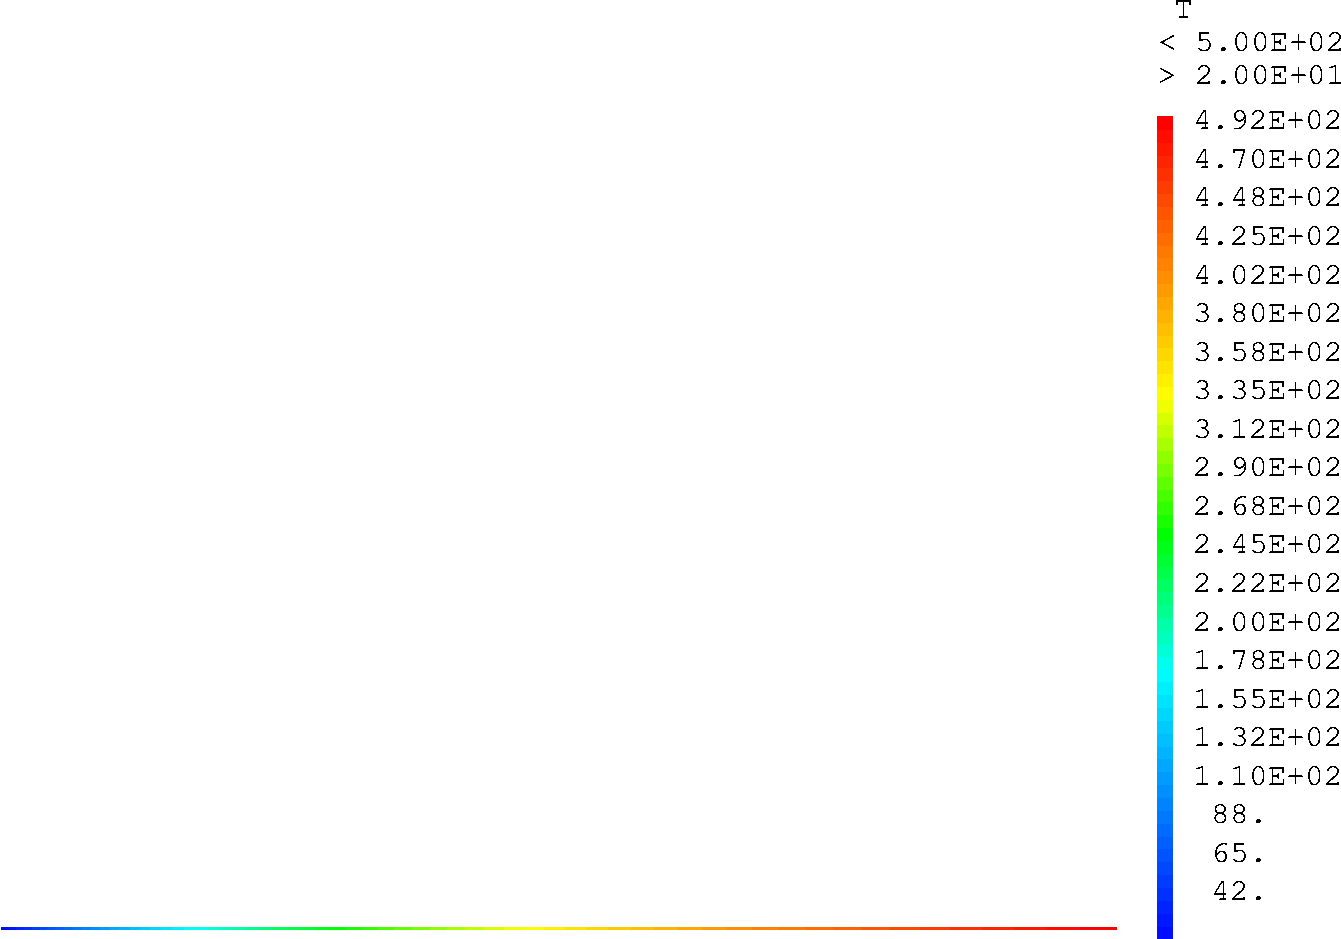
\includegraphics[width=5cm]{images/thermique_1d_axi.1}
    \end{textblock*}
    \begin{textblock*}{6cm}(6.8cm,3.5cm)
      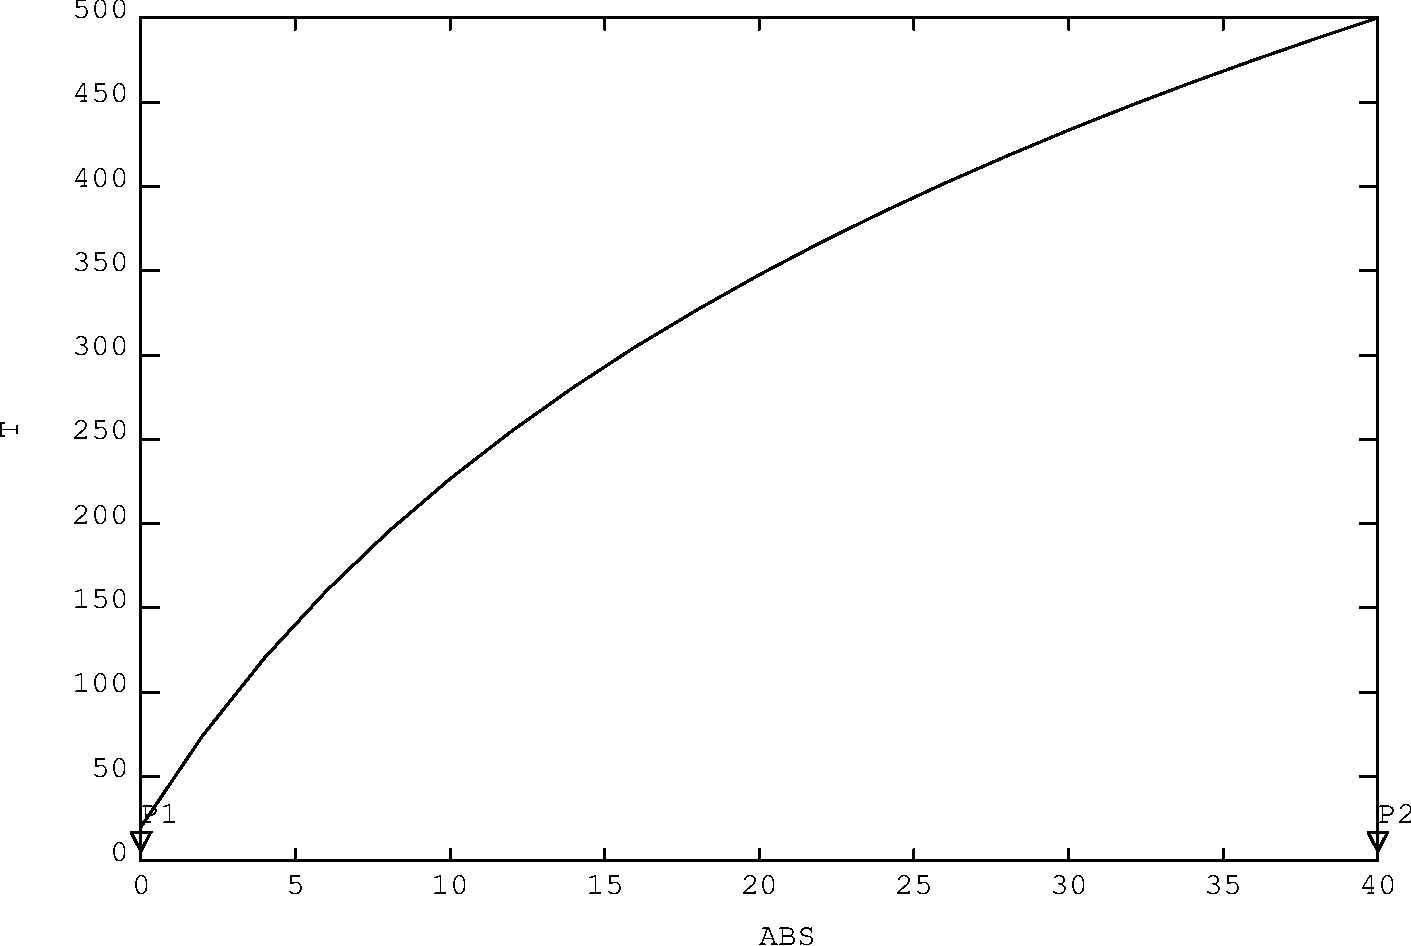
\includegraphics[width=5cm]{images/thermique_1d_axi.2}
    \end{textblock*}
    \lstinputlisting[basicstyle=\ttfamily\tiny, language=gibiane, firstline=5, lastline=26]{dgibi/thermique_1d_2d_axi.dgibi}
  \end{itemize}
  \vspace{1cm}
\end{frame}




\fe{\subsection{Entrées/Sorties}}{\subsection{Inputs/Outputs}}
\begin{frame}{\fe{Lire / Sortir des données}{Reading / Writing data}}
  \begin{itemize}
    \item \fe{\kwr{SAUV}egarder au format binaire et \kwr{REST}ituer}
             {Save and Restore data in a binary file}
    \lstinputlisting[language=gibiane, firstline=40, lastline=41]{dgibi/exemples.dgibi}
    \footnotesize
    \fe{\blue{Fichier XDR}}{\blue{XDR format}}
    \normalsize
    \item \fe{Exécuter une commande \kwr{EXTE}rieure}{Run an \kwr{EXTE}rnal command}
    \lstinputlisting[language=gibiane, firstline=43, lastline=43]{dgibi/exemples.dgibi}
    \footnotesize
    \fe{\kw{tab1} contient le résultat de la commande \kw{grep}}
       {\kw{tab1} contents the output of the \kw{grep} command}
    \normalsize
    \item \fe{\kwr{ACQU}érir un fichier texte}{\kwr{ACQU}ire any text file}\\
    \footnotesize
    \fe{Lire un fichier texte, ligne par ligne}{Read a texte file, line by line}
    \lstinputlisting[language=gibiane, firstline=45, lastline=47]{dgibi/exemples.dgibi}
    \begin{textblock*}{5cm}(6.9cm,-2cm)
      \lstinputlisting[frame=single, language=gibiane, firstline=49, lastline=51]{dgibi/exemples.dgibi}
    \end{textblock*}
    \normalsize
  \end{itemize}
\end{frame}

\begin{frame}{\fe{Lire / Sortir des données}{Reading / Writing data}}
  \begin{itemize}
    \item \fe{Écrire un fichier texte (\kwr{SORT})}{Writing a text file (\kwr{SORT})}\\
    \begin{textblock*}{7cm}(5cm,0cm)
      \lstinputlisting[basicstyle=\ttfamily\tiny, frame=single, firstline=1, lastline=21]{dgibi/fibonacci.txt}
    \end{textblock*}
    \lstinputlisting[basicstyle=\ttfamily\tiny, language=gibiane, firstline=1, lastline=17]{dgibi/fibonacci.dgibi}
  \end{itemize}
\end{frame}

\begin{frame}{\fe{Lire / Sortir des données}{Reading / Writing data}}
  \begin{itemize}
    \item \fe{Lire/Écrire des \g{\blue{données tabulées}} en colonnes}
             {Read/Write \g{\blue{tabular data}} in columns}\\
    \begin{textblock*}{2cm}(9.5cm,-1cm)
      
\includegraphics[width=1.5cm]{images/excel}
    \end{textblock*}
    \fe{\blue{Fichier .csv}}{\blue{.csv file}}\\
    \footnotesize
    \item[]\fe{Objets concernés : LISTENTI, LISTREEL, LISTMOTS, EVOLUTIO, TABLE}
              {Concerned objects: LISTENTI, LISTREEL, LISTMOTS, EVOLUTIO, TABLE}
    \item[]\fe{Utilisé par les éditeurs de texte ou tableur (Excel)}{Used by text editors or spreadsheet (Excel)}
    \lstinputlisting[language=gibiane, firstline=53, lastline=56]{dgibi/exemples.dgibi}
    \item[]
    \item[]\fe{Choix possible du séparateur de colonnes :}{The column separator can be changed:}
    \item[]\fe{point virgule, virgule, espace, tabulation, barre oblique...}{semicolon, comma, space, tab, slash}
  \end{itemize}
\end{frame}

\begin{frame}{\fe{Lire / Sortir des données}{Reading / Writing data}}
  \begin{itemize}
    \item \fe{Écrire des données au \g{\blue{format VTK}}}
             {Write data in \g{\blue{VTK format}}}\\
    \begin{textblock*}{3cm}(9.5cm,-0.3cm)
      
\includegraphics[width=2.5cm]{images/paraview}
    \end{textblock*}
    \fe{\blue{Fichier .vtk}}{\blue{.vtk file}}\\
    \footnotesize
    \item[]\fe{Objets concernés : MAILLAGE, CHPOINT, MCHAML}
              {Concerned objects: MAILLAGE, CHPOINT, MCHAML}
    \item[]\fe{Utilisé par Paraview}{Used by Paraview}
    \lstinputlisting[language=gibiane, firstline=58, lastline=59]{dgibi/exemples.dgibi}
    \normalsize
    \item \fe{Lire/Écrire des données au \g{\blue{format MED}}}
             {Read/Write data in \g{\blue{MED format}}}\\
    \begin{textblock*}{3cm}(9.5cm,-0.6cm)
      
\includegraphics[width=2.5cm]{images/salome}
    \end{textblock*}
    \begin{textblock*}{3cm}(9.5cm,0.2cm)
      
\includegraphics[width=2.5cm]{images/epx}
    \end{textblock*}
    \begin{textblock*}{3cm}(9.5cm,2cm)
      
\includegraphics[width=2.5cm]{images/aster}
    \end{textblock*}
    \fe{\blue{Fichier .med}}{\blue{.med file}}\\
    \footnotesize
    \item[]\fe{Objets concernés : MAILLAGE, CHPOINT, MCHAML, TABLE}
              {Concerned objects: MAILLAGE, CHPOINT, MCHAML, TABLE}
    \item[]\fe{Utilisé par Salomé, EuroPlexus, Code Aster}{Used by Salomé, EuroPlexus, Code Aster}
    \lstinputlisting[language=gibiane, firstline=61, lastline=64]{dgibi/exemples.dgibi}
    \normalsize
  \end{itemize}
\end{frame}

\begin{frame}{\fe{Développement : procédures Gibiane}{Development: Gibiane procedures}}
  \begin{itemize}
    \item \fe{Écrire chaque procédure dans un fichier texte :}
             {Write each procedure in a text file:}
    \begin{itemize}
      \item extension ".procedur"
      \item \fe{nom de fichier = nom de procédure}{file name = procedure name}
      \item \fe{1 fichier = 1 procédure}{1 file = 1 procedure}
    \end{itemize}
    \item \fe{Emplacements possibles :}{Location:}
    \begin{itemize}
      \item \kw{./}
      \item \kw{./procedur}
    \end{itemize}
    \item \fe{Lancer Cast3M comme d'habitude}{Launch Cast3M as usual}\\
    \kwr{castem24  } \kw{toto.dgibi}
    \item \fe{Idem pour les notices (fichiers ".notice")}
             {Idem for notices (manual pages) (".notice" files)}
  \end{itemize}
\end{frame}

\begin{frame}{\fe{Développement : sources Esope}{Development: Esope sources}}
  \begin{itemize}
    \item \fe{L'utilisateur peut modifier/corriger/ajouter le code source des opérateurs et directives}
             {The user can modify/correct/add the source code of operators and directives}
    \item \fe{Compilation des fichiers source Esope}{Compilation of Esope source files}\\
    \kwr{compilcast24  } \kw{toto.eso titi.eso ...}
    \item \fe{Édition des liens}{Linking}\\
    \kwr{essaicast24}\\
    \fe{$\Rightarrow$ création d'un fichier exécutable binaire : \g{\kwg{cast\_24}}}
       {$\Rightarrow$ creation of a binary executable file: \g{\kwg{cast\_24}}}\\
       \fe{$\Rightarrow$ version locale de Cast3M}
          {$\Rightarrow$ local version of Cast3M}
    \item \fe{Lancer Cast3M comme d'habitude}{Launch Cast3M as usual}\\
    \kwr{castem24  } \kw{toto.dgibi}
  \end{itemize}
\end{frame}

\begin{frame}{\fe{Et pour finir}{And to complete}}
  \begin{itemize}
    \item \fe{Consulter la \g{\blue{documentation}} régulièrement}
             {Peruse \g{\blue{documentation}} regularly}\\
    \footnotesize
    \fe{$\sim$ 70 instructions découvertes durant cette formation\\
        près de 1400 instructions existantes !}
       {$\sim$ 70 instructions reviewed during this course\\
        around 1400 available instructions!}\\~
    \normalsize
    \item \fe{Inscription à la \g{\blue{liste de diffusion Cast3M}} (voir le site web Cast3M)}
             {Subscription to the \g{\blue{Cast3M mailing list}} (see the Cast3M web site)}\\
    \footnotesize
    \fe{Envoyer un e-mail vide à \href{mailto:sympa@umontpellier.fr}{\kw{sympa@umontpellier.fr}}\\
        avec comme objet du message :}
       {Send an e-mail at \href{mailto:sympa@umontpellier.fr}{\kw{sympa@umontpellier.fr}}\\
        with in the message frame:}
    \begin{center}
      \kw{SUB  cast3m-util last\_name  first\_name}
    \end{center}
    \fe{et rien d'autre ! (pas de message, pas de signature, …)}
       {and nothing more! (no object, no signature, …)}\\~
    \normalsize
    \item \fe{\g{\blue{Club Cast3M}} : séminaire annuel des utilisateurs}
             {\g{\blue{Club Cast3M}}: annual users seminar}\\
    \footnotesize
    \fe{Chaque année en novembre dans le sud de Paris\\
        Présentation de travaux réalisés avec Cast3M, nouveautés de la prochaine version\\
        Inscription gratuite !}
       {Each year in November in the south of Paris\\
        Presentation of studies performed with Cast3M, developments in the next release\\
        Free registration!}
  \end{itemize}
\end{frame}
